
\documentclass[ms.tex]{subfiles}
\begin{document}

\section{Results}
\label{sec:results}

\subsection{Evolution of a Fiducial Model}
\label{sec:results:fiducial}

\begin{figure*}
\centering
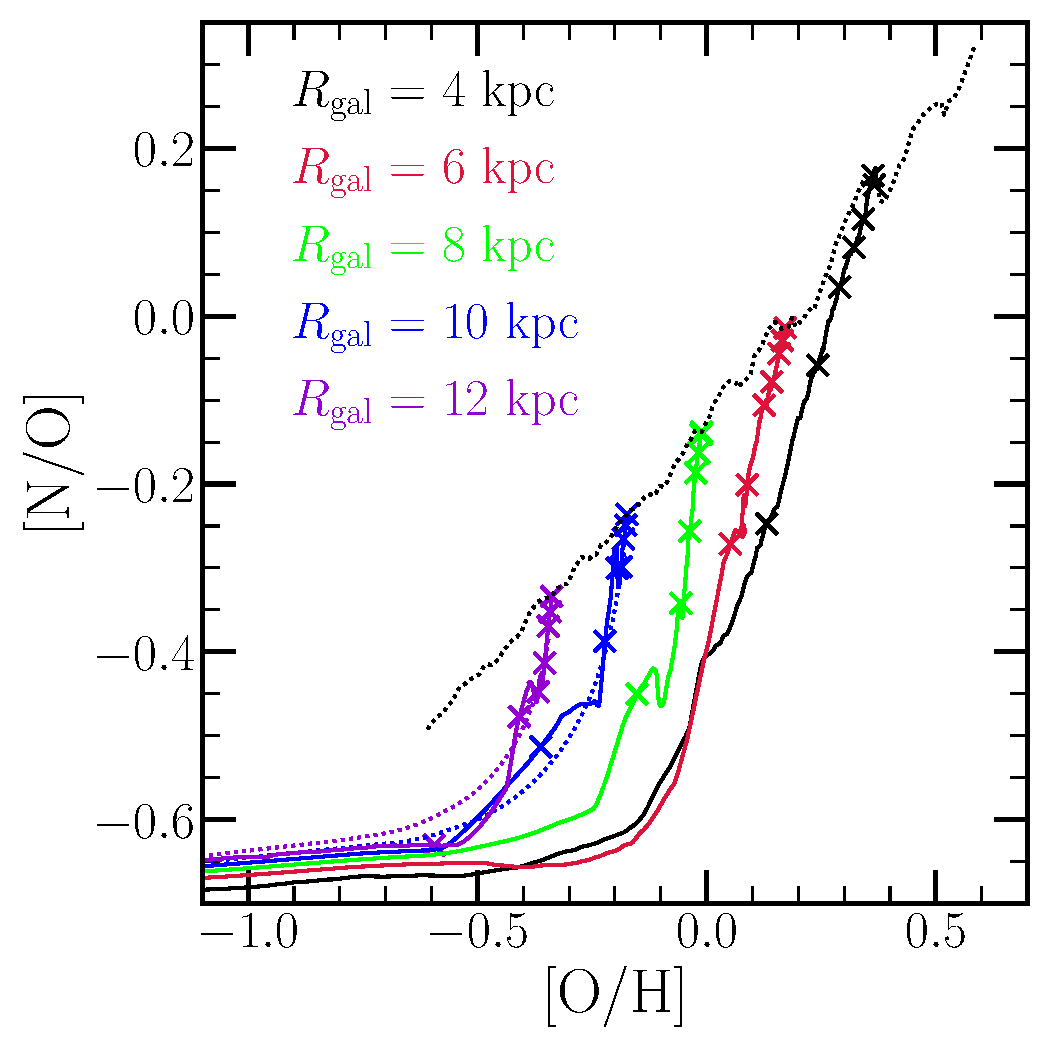
\includegraphics[scale = 0.45]{no_oh_superposition.pdf}
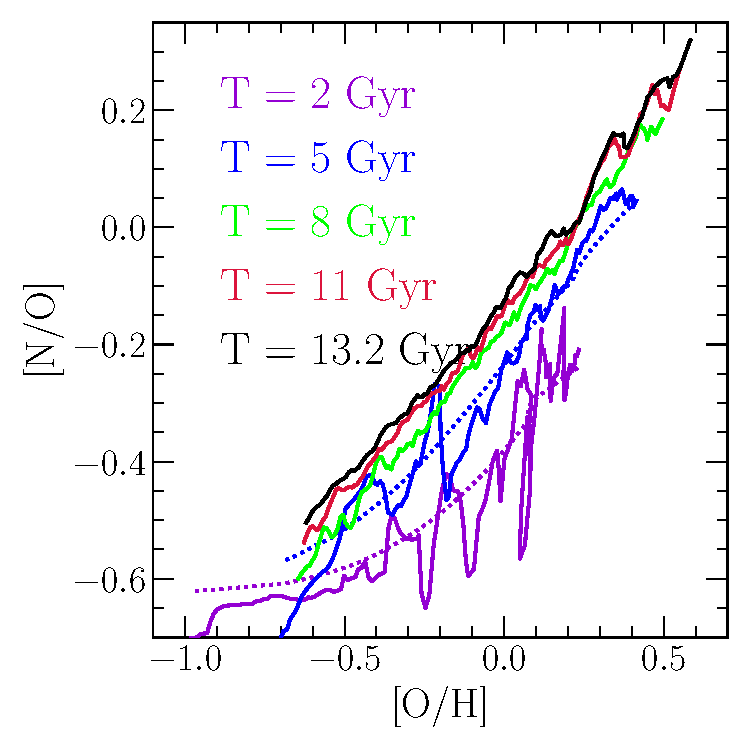
\includegraphics[scale = 0.45]{no_oh_timeevol.pdf}
\caption{
\textbf{Left}: The gas-phase~\ohno~relation parameterized by time at
fixed radius (solid coloured lines) in the fiducial model. X's denote the
abunadnces at~$T = 2$, 4, 6, 8, 10, 12, and 13.2 Gyr (the present day) at all
radii.
The dotted black line is the same as the solid black line in the right panel.
Coloured dotted lines mark the evolution of our model at~$\rgal = 10$ and 12
kpc when stellar migration is neglected (i.e. the ``post-processing'' migration
model from~\citealp{Johnson2021}).
\textbf{Right}: The gas-phase~\ohno~relation parameterized by radius at
various snapshots (solid coloured lines) in our fiducial model.
Similar to the left panel, coloured dotted lines denote the resulting relation
at~$T = 2$ and 5 Gyr when we neglect stellar migration.
}
\label{fig:no_oh_timeevol}
\end{figure*}

Our fiducial model adopts, together with the SN yields of
\citet[][see discussion in~\S~\ref{sec:yields:ccsne}]{Johnson2021},
$y_\text{N}^\text{CC} = 3.6\times10^{-4}$ and our linear AGB star yield model
with~$\xi = 9\times10^{-4}$.
Although we presented this model in comparison to the~\cristallo~yields with
$\xi = 3\times10^{-4}$ in~\S~\ref{sec:yields:agb}, we find that a
renormalization of this model is necessary to reproduce the~\ohno~relation as observed with the~\citet{Johnson2021} GCE model.
We discuss this point further in~\S~\ref{sec:results:yields}.
To demonstrate the impact of stellar migration on N enrichment rates, we make
use of the ``diffusion'' migration model in this section (see discussion
in~\S~\ref{sec:multizone}).
\par
In the left panel of Fig.~\ref{fig:no_oh_timeevol}, we plot the evolution of N
and O abundances in the gas phase at five different Galactocentric radii.
At early times,~\oh~is low and~\no~reflects the ratio of the CCSN yields
(\no\subcc~$\approx -0.7$).
Consequently, the tracks in each ring are similar.
Once lower mass stars begin to evolve through an AGB phase, they enrich the
interstellar medium (ISM) with N but negligible amounts of O, increasing~\no.
At this point, the tracks in each ring separate from one another.
This separation is a consequence of the metallicity gradient in~\oh~being
established early in the Galaxy's evolution.
Being an element produced primarily by CCSNe on short delay times, O reaches
an equilibrium abundances on timescales of a~$\sim$few Gyr~\citep{Weinberg2017}.
Each ring therefore achieves equilibrium in O soon after AGB stars begin
producing N, after which~\no~continues to increase at an approximately
fixed~\oh.
The separation of these evolutionary tracks further suggests that
the~\ohno~relation arises not as an evolutionary sequence but as a
superposition of endpoints.
That is, the relation that would be derived observationally for this model
taking the N and O abundances at the present day from all rings (shown by the
dotted black line; see discussion below) does not reflect the N and O
abundances of the Galaxy in the past.
Similar arguments have been made regarding low [$\alpha$/Fe] disc stars
\citep[e.g.][]{Schoenrich2009, Sharma2020}.
\par
Because there is a delay between a stellar population's formation and N
production from its AGB stars ($\sim$250 Myr in this model; see Fig.
\ref{fig:ssp}), stellar migration can in principle occur within this time
interval.
Although the bulk of migration occurs on longer timescales, this characteristic
delay is comparable to the dynamical time of the Milky Way and is thus adequate
for kinematic heating to at least begin.
As a consequence, there may be a slight deficit or surplus of N-producing AGB
stars in a given ring at some time induced by stellar migration.
These tracks can thus move vertically in this plane in response to AGB stars
moving between rings as the Galaxy evolves, entirely independent of the SFH and
the nucleosynthetic yields of stars than formed at a given radius and time.
We demonstrate this effect by comparing the solid blue and purple lines to
their dotted counterparts, which denote the tracks when we neglect the impact
of stellar migration on enrichment rates (i.e. the ``post-processing'' model
from~\citealp{Johnson2021}).
% This is qualitatively similar to what~\citet{Johnson2021} find for SN Ia
% enrichment of Fe (see discussion in their~\S\S~3.1 and 3.4).
\par
In the right panel of Fig.~\ref{fig:no_oh_timeevol}, we plot the
gas-phase~\ohno~relation predicted by the model at various snapshots.
To obtain this, we simply take the N and O abundances in the ISM at a given
output time for each~$\delta\rgal = 100$ pc ring at~$\rgal > 2$ kpc and plot
them as a line.
The relation is generally time-independent at~$T \gtrsim 5$ Gyr, though there
is some slight evolution toward higher~\no.
We again demonstrate the impact of stellar migration by comparing the blue and
purple solid lines to their dotted counterparts, which quantify the relation
when we neglect stellar migration.
This indicates that the complex features seen in the relation at all times are
a consequence of migration as discussed above.
\par
The mechanism by which stellar migration imposes complex features in
the~\ohno~plane is qualitatively similar to what~\citet{Johnson2021} find for
SN Ia production of Fe (see discussion in their~\S\S~3.1 and 3.4).
They found that the SN Ia rate in this model can vary by as much as a factor of
$\sim$3 at large radii ($\rgal \gtrsim 9$ kpc).
As a consequence, some of the resultant stellar populations are Fe-poor enough
to present as young stars ($\lesssim$ 6 Gyr) with significantly super-solar
[$\alpha$/Fe] ratios.
Stars with these ages and chemical compositions have indeed been observed in
the solar neighbourhood with APOGEE\footnote{
	Apache Point Observatory Galaxy Evolution Experiment~\citep{Majewski2017}.
}~\citep{Chiappini2015, Martig2015, Martig2016, Warfield2021}.
Although a substantial portion of these stars appear to have undergone mass
transfer from a binary companion, making them appear younger than they truly
are~\citep{Jofre2016, Yong2016, Izzard2018, SilvaAguirre2018, Miglio2021}, some
exhibit [C/N] ratios consistent with truly young ages~\citep{Hekker2019}.
\citet{Johnson2021} argue that the impact of stellar migration on enrichment
rates is responsible for this intrinsically young sub-component.
In the case of N, the effect is much smaller ($\lesssim$ 0.1 dex in~\no),
but Fig.~\ref{fig:no_oh_timeevol} suggests there are some instances at early
times where the effect is more substantial.
Stellar migration's smaller effect on N enrichment rates compared to Fe can be
understood from the relative timescales of their production (see Fig.
\ref{fig:ssp} and discussion in~\S~\ref{sec:yields:imf_agb}).
Our model predicts N yields to be ejected from stellar populations~$\sim$5
times faster than Fe (even faster in our alternate yield models with larger
contributions from high mass AGB stars).
Consequently, there is much less time for stellar migration to occur within the
timescale of N production than there is within the timescale of Fe production.
This underscores the argument from~\citet{Johnson2021} that in order for
nucleosynthetic yields to migrate significant distances along with their
progenitor stellar populations, the timescale for production needs to be at
least comparable to the migration timescale.

\subsection{Comparison to Observed Gas Phase Trends}
\label{sec:results:yields}

\begin{figure*}
\centering
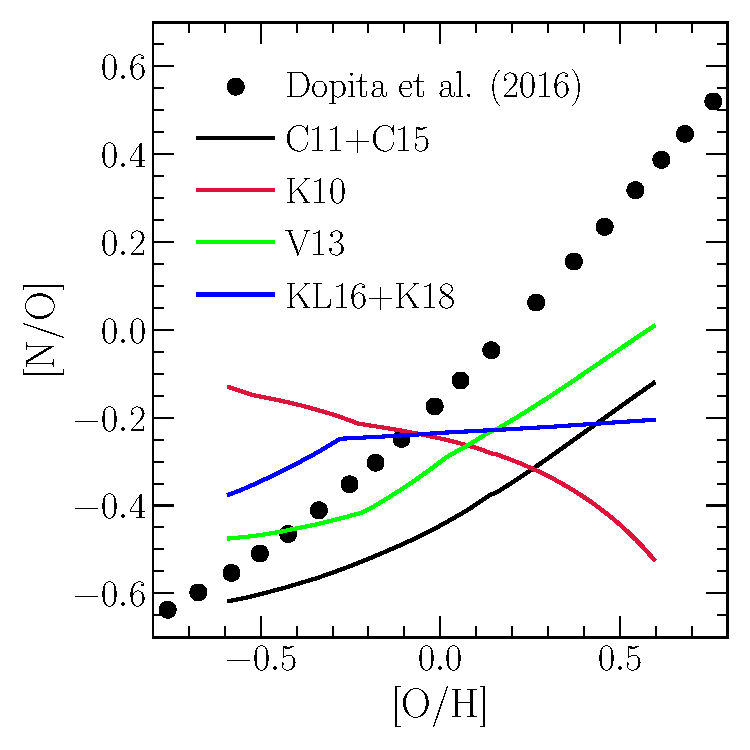
\includegraphics[scale = 0.32]{no_oh_predictions_unmodified.pdf}
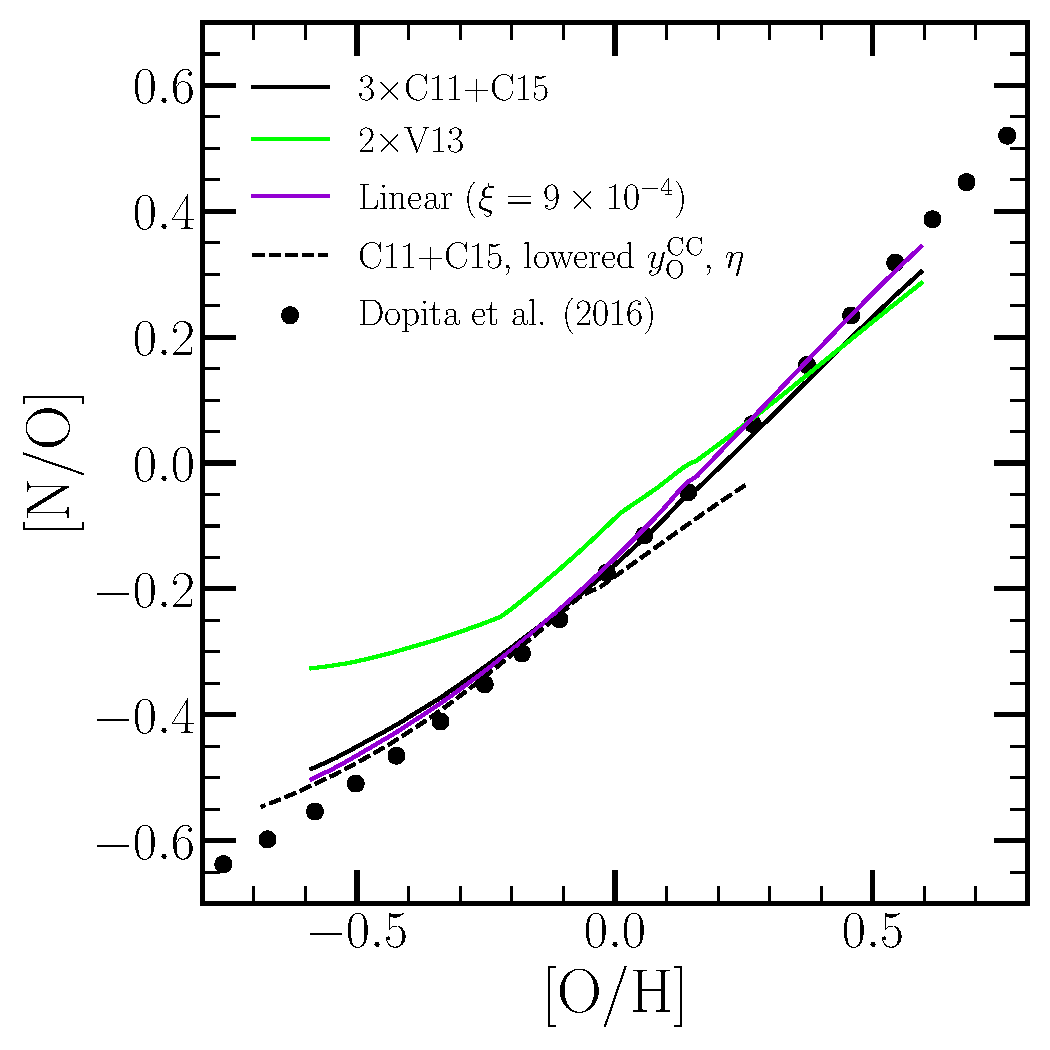
\includegraphics[scale = 0.32]{no_oh_predictions.pdf}
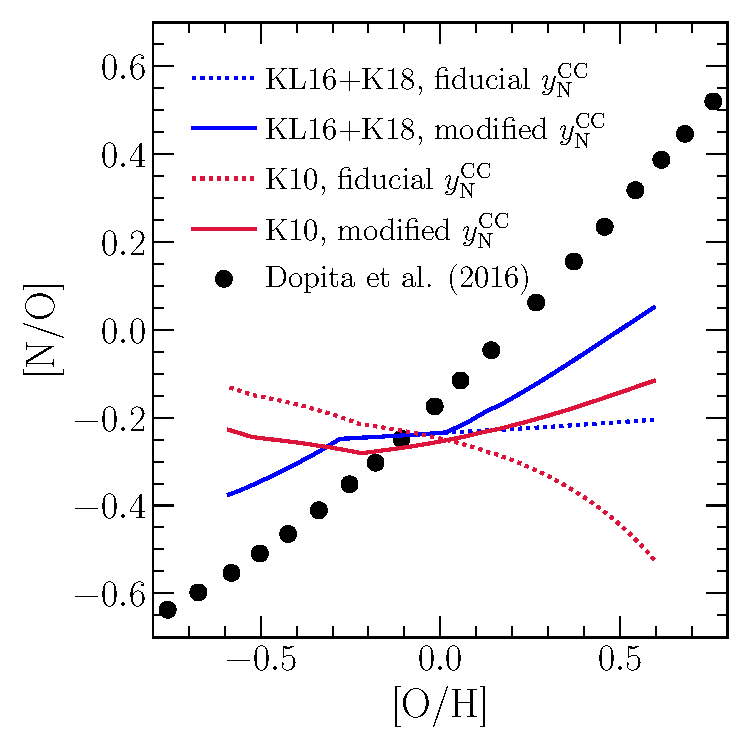
\includegraphics[scale = 0.32]{no_oh_predictions_karakas.pdf}
\caption{
\textbf{Left}: The present-day gas-phase~\ohno~relation predicted by our
model with each of the four yield models based on stellar evolution models
discussed in~\S~\ref{sec:yields:agb}, colour-coded according to the legend.
We include the~\citet{Dopita2016} measurements of this relation for local stars
and HII regions (duplicated from Fig.~\ref{fig:no_oh_observed}) as the
observational benchmark.
\textbf{Middle}: The same as the left panel, but for a case where we
artificially amplify the~\cristallo~yields by a factor of 3 and
the~\ventura~yields by a factor of 2.
We include our linear model as well, but with the slope amplified from
$\xi = 3\times10^{-4}$ as shown in Fig.~\ref{fig:agb_yield_models} to
$\xi = 9\times10^{-4}$ since it is also based on the~\cristallo~yields.
\textbf{Right}: The same as the left panel, but comparing the predictions made
by the~\karakasten~and~\karakas~yields with our fiducial value of
$y_\text{N}^\text{CC}$ (dotted lines, same as left-hand panel) to those with
alternate forms of~$y_\text{N}^\text{CC}$ (solid lines; see discussion in~\S
\ref{sec:results:yields}).
We show all predictions with ``post-processing'' migration model (see
discussion in~\S~\ref{sec:multizone}).
}
\label{fig:no_oh_predictions}
\end{figure*}

We use the~\citet{Dopita2016} measurements as our observational benchmark.
They are a good representation of many results for gas phase N and O abundances
(see Fig.~\ref{fig:no_oh_observed}), and they agree well with APOGEE stellar
trends~\citep{Vincenzo2021}.
To make the comparison between different yield models more clear, we neglect
the impact of stellar migration on enrichment rates and make use of the
``post-processing'' migration model in this section (see discussion in~\S
\ref{sec:multizone}).
\par
In the left panel of Fig.~\ref{fig:no_oh_predictions}, we compare the
predictions of our multi-zone GCE model with each of the AGB star yield tables
predicted from stellar evolution models (see Fig.~\ref{fig:agb_yield_models}
and discussion in~\S~\ref{sec:yields:agb}).
Since it is based on the~\cristallo~yields, we find similar results with our
linear model with a slope of~$\xi = 3\times10^{-4}$.
All four AGB star yield models fail to reproduce the gas-phase~\ohno~relation
as observed.
The~\cristallo~and~\ventura~yields are able to reproduce the qualitative trend,
but with an incorrect normalization.
The~\karakasten~and~\karakas~yields, on the other hand, fail to reproduce
the steadily sloped increase of~\no~with~\oh.
\par
In order to successfully reproduce the observations, we find that we need to
artificially amplify the~\cristallo~and~\ventura~yields by factors of~$\sim$3
and~$\sim$2, respectively.
Having originally compared our linear model to the~\cristallo~yields in
Fig.~\ref{fig:agb_yield_models} with a slope of~$\xi = 3\times10^{-4}$, we
amplify this value by a factor of 3 here as well.
We illustrate the results of these modified yield models in the middle panel
of Fig.~\ref{fig:no_oh_predictions}.
Although the~\ventura~model predicts an~\ohno~relation that is slightly
shallower than the~\citet{Dopita2016} measurements, the predictions are
reasonably within the scatter seen in Fig.~\ref{fig:no_oh_observed}.
Rather than artificially amplifying the~\cristallo~and~\ventura~yields, we also
find good agreement with the observed relation if we lower both our SN yields
and our outflow mass loading factor~$\eta$ as a function of~\rgal~by similar
factors from their values in~\citet{Johnson2021}.
These parameters, which approximately determine the equilibrium abundance in a
one-zone model~\citep{Weinberg2017}, are tuned to reproduce a metallicity
gradient in the disc that resembles that observed for the Milky Way (see
discussion in~\S~2.4 of~\citealp{Johnson2021}).
However, since the yield and the outflow are simply source and sink terms in
computing enrichment rates, the model makes similar predictions when both are
lowered by the same factor.
We demonstrate this point in the middle panel of Fig.
\ref{fig:no_oh_predictions} with the black dashed line for the~\cristallo~model
with both~\ycc{O}~and~$\eta$ each lowered by a factor of 3.
This model spans a different range in~\oh~because the relation between~\ycc{O},
$\eta$, and the equilibrium abundance is only approximately one-to-one, but the
predictions also exhibit good agreement with the~\citet{Dopita2016}
measurements.
\par
Lowering our SN yields by a factor of~$2 - 3$ is plausible if a substantial
fraction of massive stars collapse directly to black holes as opposed to
exploding as SNe at the ends of their lives.
Our IMF-averaged massive star yields (see discussion in~\S
\ref{sec:yields:ccsne}) are based on a~\citet{Kroupa2001} IMF combined with SN
nucleosynthesis models in which most~$M > 8~\msun$ stars explode as a CCSN
\cite[e.g.][]{Woosley1995, Chieffi2004, Chieffi2013, Limongi2018, Nomoto2013},
but recent results contest the validity of this assumption.
The criteria for massive star explosions and which stars of what masses end
their lives in ``failed supernovae'' has been a recent topic of interest from
both theoretical~\citep[e.g.][]{Pejcha2015, Sukhbold2016, Ertl2016} and
observational perspectives (e.g.~\citealp*{Gerke2015};~\citealp{Adams2017,
Basinger2021}).
At present, no combination of a SN nucleosynthesis model with a physically
motivated black hole landscape is able to reproduce the observed abundance
patterns~\citep{Griffith2021}.
Despite this, black hole formation still lowers SN yields by simply not
producing explosive nucleosynthetic products and is thus an alternate
explanation for the failure of our fiducial model to reproduce the
observed~\ohno~relation with the~\cristallo~and~\ventura~yield models.
With~\vice's~\texttt{vice.yields.ccsne.fractional} function, designed to
calculate values of~\ycc{X}~for various elements (see discussion in~\S
\ref{sec:yields:ccsne} here and in~\S~4 of~\citealp{Griffith2021}), we indeed
find a value of~$\ycc{O} = 0.0056$ using the W18 explosion model from
\citet{Sukhbold2016} compared to our fiducial value of~$\ycc{O} = 0.015$.
\par
Alternatively,~\citet{Vincenzo2016a} are able to reproduce the~\ohno~relation
in chemical evolution models with the~\ventura~yields by implementing a
differential wind in which outflows remove O but not N from the star forming
gas reservoir.
Because the enrichment rates are the same as in our models with lowered SN
yields, we again find similar results if simply add a portion of the SN yields
(both CCSN and SN Ia) to the outflow while still lowering~$\eta$ at all radii.
If SNe are the sources of outflow-driving winds, such a scenario is suggested
by recent observational~\citep*{Chisholm2018} and theoretical arguments
\citep{Christensen2018}, and could also account for this difference in our
fiducial model if AGB stars do not significantly contribute to driving outflows.
\par
With the~\karakasten~and~\karakas~models failing to reproduce the qualitative
trend of~\no~with~\oh, none of the variations discussed above in the
context of the~\cristallo~and~\ventura~yields are able to reproduce the
observed results.
Each of these alternate parameterizations corresponds to a renormalization of
the predicted~\ohno~relation, and with inaccurate slopes, there is no factor by
which the predicted~\no~ratios predicted by either~\karakasten~or~\karakas~can
be amplified or diminished in order to accurately explain the data.
However, in principle it is possible that a metallicity-dependent CCSN yield of
N could make up the difference.
\par
If the~\karakasten~yields are to reproduce the observations, the overall N
abundance must decrease at low~\oh~and increase at high~\oh.
We therefore construct the following parameterization of~\ycc{N}:
\begin{equation}
\ycc{N} = (3.6\times10^{-4})\left(\frac{Z}{Z_\odot}\right),
\label{eq:linear_yncc}
\end{equation}
where~$Z_\odot$ is the total metallicity of the sun, for which we take a value
of~$Z = 0.014$ based on the findings of~\citet{Asplund2009} and
\citet*{Asplund2021}.
We illustrate this CCSN yield model with the slanted black dotted line in the
left hand panel of Fig.~\ref{fig:n_cc_yields}.
While our fiducial value of~$\ycc{N} = 3.6\times10^{-4}$ best describes the
rotating CCSN progenitor models of~\citet{Limongi2018}, this alternate
parameterization follows the non-rotating models published in
\citet{Limongi2018},~\citet{Sukhbold2016},~\citet{Nomoto2013}, and
\citet{Woosley1995} while maintaing the same base-line value of
$3.6\times10^{-4}$ at solar metallicity.
If the~\karakas~yields are to reproduce the observations, then contrary to the
predictions made with the~\karakasten~yields, the~\no~ratio at low~\oh~is
fine (albeit slightly high by~$\sim$0.2 dex).
Instead, only the N abundance at high~\oh~needs correcting.
We therefore construct a second alternate form of~\ycc{N}~by retaining the
value of the fiducial yield at sub-solar metallicity but assuming the value of
equation~\refp{eq:linear_yncc} at super-solar abundances:
\begin{equation}
\ycc{N} = (3.6\times10^{-4})\max\left(1, \frac{Z}{Z_\odot}\right).
\label{eq:broken_yncc}
\end{equation}
\par
We compare our GCE model predictions with these alternate CCSN yield
parameterizations for the~\karakasten~and~\karakas~AGB star yield models in
the right-hand panel of Fig.~\ref{fig:no_oh_predictions}.
These metallicity-dependent CCSN yields are able to make up some of the
difference, but both models still predict an~\ohno~relation that is simply
too shallow to explain the observations.
The inverse dependence of~\no~with~\oh~with our fiducial CCSN yield and
the~\karakasten~AGB star yields can be understood by the interaction between
TDU and HBB (see discussion in~\S~\ref{sec:yields:agb}).
Both effects are stronger at low metallicity, and since all of
the~\karakasten~stars experiencing HBB also experience TDU (see their Table 1),
such a result is unsurprising.
This is also true for the~\karakas~yields, but that model predicts a relatively
flat~\ohno~relation owing to differences in the~\Nfourteen~yields as a
consequence of updates model inputs regarding opacity and mass loss (see
discussion in~\S~\ref{sec:yields:agb}).
In principle, there are parameterizations of~\ycc{N}~which could reproduce
the~\ohno~relation with the~\karakasten~and~\karakas~yield models - whatever
makes up the difference at a given~\oh~can be assumed to be the corresponding
CCSN yield.
Such assumptions, however, would be challenged by both the rotating and the
non-rotating SN nucleosynthesis models illustrated in
Fig.~\ref{fig:n_cc_yields}.
Despite these results, we cannot say with any confidence whether or not such
a wide mass range of stars should experience both TDU and HBB during the AGB
phase as in~\karakasten~and~\karakas.
Although this makes it difficult for these models to predict a monotonic
increase of~\no~with~\oh, there are many uncertain parameters required to
predict yields from stellar evolution models, and we have only investigated a
few of them here.
\par
In short, we find that in order to reproduce the gas-phase~\ohno~relation as
observed, our model requires the sum total N yields from both CCSNe and AGB
stars to scale roughly linearly with metallicity.
Assuming our fiducial value of~$\ycc{N} = 3.6\times10^{-4}$, we previously
illustrated this dependence in the right panel of Fig.~\ref{fig:ssp}.
With the~\cristallo~and~\ventura~models specifically, our results suggest that
these yields must increase by factors of~$2 - 3$ or that many massive stars
stars must collapse directly to black holes; it may also be some mix of the
two.


\subsection{Comparison to Stellar Abundances in the Milky Way Disc}
\label{sec:results:vincenzo_comp}

\subsection{The Sources of Scatter in the~\ohno~Relation}
\label{sec:results:schaefer_comp}

\end{document}

